After conducting the measurements, profiles showing the drag coefficient as a function of the wind velocity could be created for each set of disks, as well as for the rotating WT models. In this section, the drag and drag coefficient profiles are presented and discussed, as well as the calculated average Cd and the standard deviations. In the end, the measurement noise is discussed. 




\section{Rotational WT model}

The first measurement conducted using three rotating WT models resulted in a drag coefficient that was relatively independent of wind velocity for four of the measured wind velocities, but with a significant deviation at 5 m/s. To investigate whether this deviation was due to a measurement error, a second measurement was conducted, this time using three new rotating WT models. This second measurement gave more of an expected result at 5 m/s, however showed a deviation at 15 m/s. Thus, a third measurement, once again with three new rotating WT models, was conducted. Finally, a fourth measurement was carried out, this time using the same models as during the third measurement. The resulting drag coefficients can be seen as a function of wind velocity in figure \ref{fig:RotationalCD}.

\begin{figure}[h!]
    \centering
    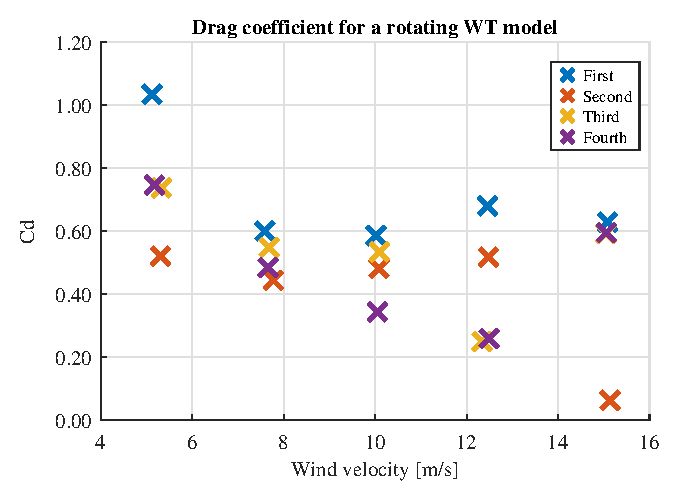
\includegraphics[width=\linewidth]{0_Images/RotationalCD.eps}
    \caption{The drag coefficient for the rotating WT models, obtained through four rounds of measurements.}
    \label{fig:RotationalCD}
\end{figure}

As can be seen, there is some variation between the different measurements. The values from the third and the fourth measurement, conducted using the same WT models, are quite similar at 5 m/s, 7.5 m/s and 12 m/s, and at 15 m/s, they completely overlap. This may show that the measurement is repeatable, and that one of the reasons for the varying results is simply that the rotating WT models have small differences, for example related to the friction of the rotating blades and how well they are connected. Be it too tight, there will be added friction. Be it too loose, the blades may start to oscillate. However, even between the third and fourth measurement, there is a noticeable difference at 7.5 m/s, showing that differences between the WT models is not the only cause for the varying results. 

Other possible causes of this variation may be related to noise and fluctuations in the applied wind velocity and in the force plate. 
%HOW CAN THIS BE EXPLAINED 

To investigate the results further, the drag resulting from the different measurements are pictured as a function of wind velocity in figure \ref{fig:RotationalDrag}


\begin{figure}[h!]
    \centering
    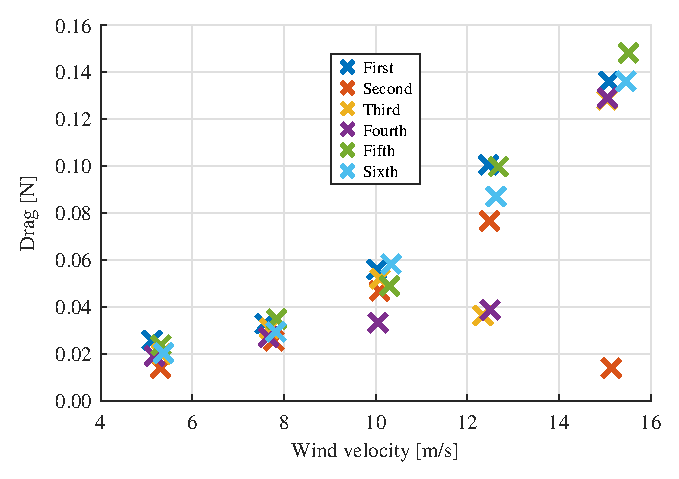
\includegraphics[width=\linewidth]{0_Images/RotationalDrag.eps}
    \caption{The measured drag for the rotating WT models, obtained through four rounds of measurements.}
    \label{fig:RotationalDrag}
\end{figure}

The drag at 12.5 m/s is lower than the drag at 10 m/s for the third measurement set, and the drag at 15 m/s is lower than the drag for 12.5 m/s for the second measurement set. This is not physical, and thus it is assumed that these two values are errors. The drag measured during the fourth measurement coincides with the disregarded drag from the third measurement, and is thus also regarded as an outlier. The wind tunnel did, for some unknown reason, seem to produce larger amounts of noise on the signal for velocities between 11 and 13 m/s, which might explain this repeated deviation. The drag at 10 m/s for the fourth measurement is higher than the drag at 7.5 m/s, however the value is lower than for all the measurements which seem to coincide quite well, and thus this value is considered as an outlier. The initial suspicious value, measured at 5 m/s in the first measurement, results in a $C_d$ larger than one, which seems unlikely, and hence this value is also regarded as an outlier. 
%AGREE? 

The outlier seem to be spread out both in terms of velocity at which they occur and in terms of whether they exceed or fall below the other values. One can argue that if taking a large number of new measurements, they would have a Gaussian distribution about a mean, and that taking the average of the values that seemingly coincide would be representative for this total mean. %Should probably be extended 

Thus, in order to achieve a representative value for the drag coefficient of the rotating WT models, the outliers were removed, and the average of the remaining drag coefficients was taken. This resulted in the drag coefficients seen in figure \ref{fig:RotationalAvg}.

\begin{figure}[h!]
    \centering
    \includegraphics[width=\linewidth]{0_Images/RotationalAverage.eps}
    \caption{The average drag coefficient for the rotational WT models for each wind velocity, based on the four conducted measurements, after removing the assumed wrongful outliers.}
    \label{fig:RotationalAvg}
\end{figure}

Assuming that $C_d$ is Reynolds number independent for such a short span at Reynolds numbers, the average over these measurement points is taken, resulting in an average $C_d$ of 0.585. Based on all the applied values, the standard deviation at hand is... Thus, when creating the ADs, this is the desired drag coefficient. 



\section{Drag on the ADs}
%kommenter at me uansett bryr oss mest om 10m/s, som e i den stabile delen 

The drag coefficient on the produced ADs has been studied. Initially, the solid disk, used as a reference case, produced the drag seen in figure \ref{Fig:SolidDrag} and the drag coefficient seen in figure \ref{Fig:SolidCD}. Further, the drag and the drag coefficient for the two types of disks with 60\% solidity can be seen in figure \ref{Fig:SixtyDrag} and \ref{Fig:SixtyCD}, respectively. For all three disks, the drag is seen to increase with increasing wind velocity, as one would expect. The average drag coefficient and the standard deviation is presented in table \ref{tab:AvgCD}.


\begin{figure} [h!]
    \centering
    \begin{subfigure}[b]{0.45\linewidth}
        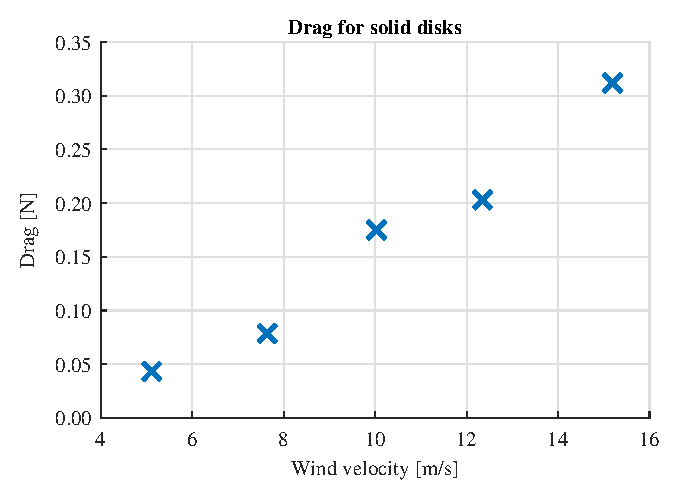
\includegraphics[width=\textwidth]{0_Images/SolidDrag.eps}
        \caption{The drag.}
        \label{Fig:SolidDrag}
    \end{subfigure}
    ~
    \begin{subfigure}[b]{0.45\linewidth}
        \includegraphics[width=\textwidth]{0_Images/SolidCD.eps}
        \caption{The drag coefficient.}
        \label{Fig:SolidCD}
    \end{subfigure}
    \caption{Using the solid disk.}
    \label{fig:SolidDisk}
\end{figure}


\begin{figure} [h!]
    \centering
    \begin{subfigure}[b]{0.45\linewidth}
        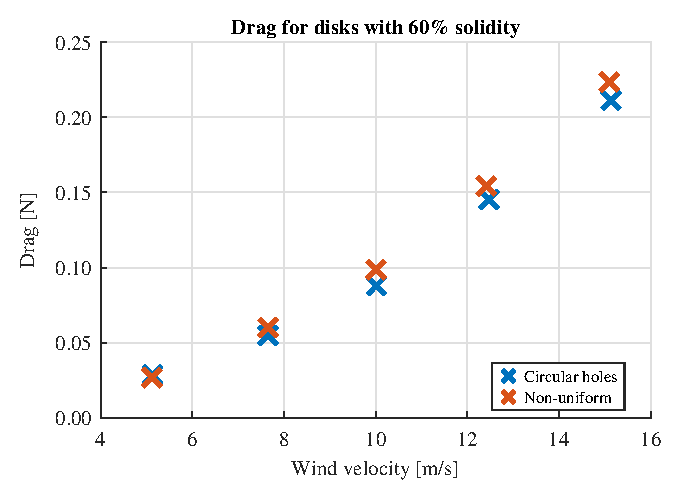
\includegraphics[width=\textwidth]{0_Images/SixtyDrag.eps}
        \caption{The drag.}
        \label{Fig:SixtyDrag}
    \end{subfigure}
    ~
    \begin{subfigure}[b]{0.45\linewidth}
        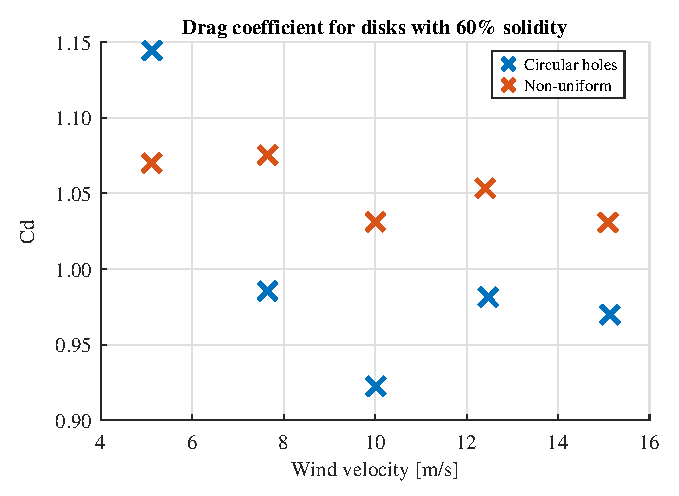
\includegraphics[width=\textwidth]{0_Images/SixtyCD.eps}
        \caption{The drag coefficient.}
        \label{Fig:SixtyCD}
    \end{subfigure}
    \caption{Using the disks with 60\% solidity.}
    \label{fig:SixtyDisk}
\end{figure}

\FloatBarrier

Further, the drag and drag coefficient for the disks with 40\% and 35\% solidity were plotted in figure \ref{fig:FortyDrag} and \ref{fig:FortyCD}. As these disks produced a drag coefficient fairly close to the average drag coefficient of the rotating turbines, this value is also included in the plots. The average drag coefficient and standard deviation can be seen in table \ref{tab:AvgCD}. 

\begin{figure}[h!]
    \centering
    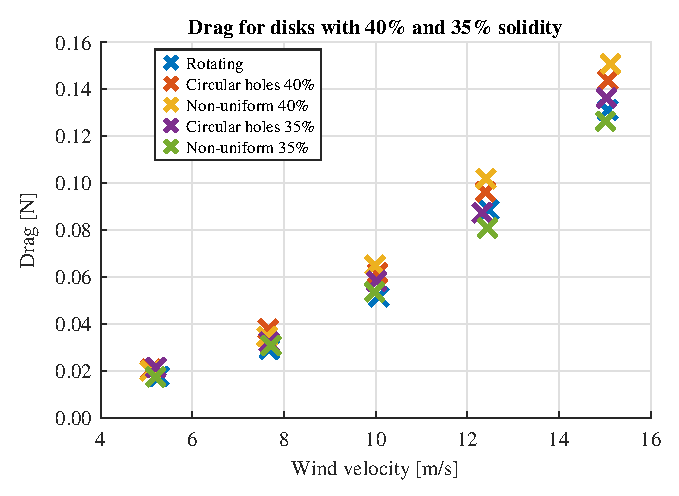
\includegraphics[width=\linewidth]{0_Images/FortyDrag.eps}
    \caption{The drag for the disks with 40\% and 35\% solidity, compared to the average drag coefficient of the rotating disks.}
    \label{fig:FortyDrag}
\end{figure}

\begin{figure}[h!]
    \centering
    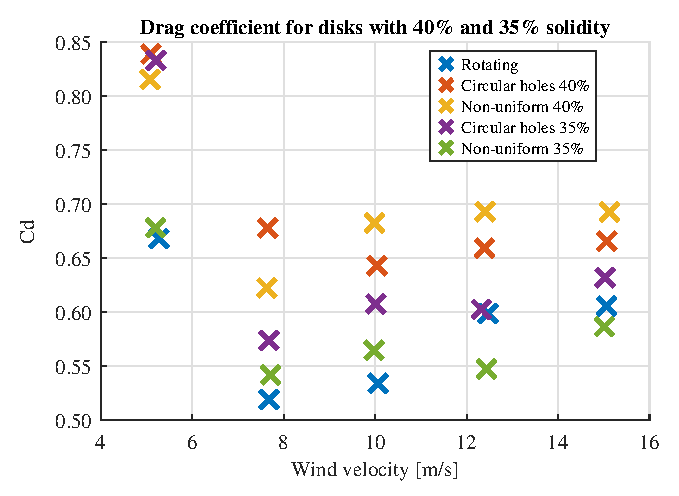
\includegraphics[width=\linewidth]{0_Images/FortyCD.eps}
    \caption{The drag coefficient for the disks with 40\% and 35\% solidity, compared to the average drag coefficient of the rotating disks.}
    \label{fig:FortyCD}
\end{figure}


Some general trends can be observed. For all disks presented in figure \ref{fig:FortyCD}, as well as for the disk with circular holes at 60\% solidity in figure \ref{Fig:SixtyCD}, Cd measured at 5 m/s is significantly higher than for the other velocities, while the measurements at the four other velocities seem to concentrate around some mean value. This may be a result of ... 


\begin{table}[H]
    \centering
    \begin{tabular}{l c c r}
         Disk type & Average Cd & SD \\
         \hline
         Rotating average & 0.5853 &  \\
         Solid & 1.5596 &  \\
         Uniform holes, 60\% & 1.0007 & \\
         Non-uniform, 60\% & 1.0521 &  \\
         Uniform holes, 40\% & 0.6970 &  \\
         Non-uniform, 40\% & 0.7013 &  \\
         Uniform holes, 35\% & 0.6499 & \\
         Non-uniform, 35\% & 0.5840 &  \\
    \end{tabular}
    \caption{Average Cd for each disk.}
    \label{tab:AvgCD}
\end{table}

%for last one, 0.5843 without drift 

In terms of these results, the non-uniform disk can be seen to produce a slightly higher drag at the same solidity compared to the uniform disk at 60\% and 40\% solidity. The same trend can not be seen at 35\% solidity, however this design with holes is created in a different way, with a larger circumference, and may not be exactly comparable. The non-uniform 35\% disk seems to best match the rotating WT model. 

As can readily be seen, the drag coefficient decreases with decreasing solidity, as one would expect. This can be compared to \cite{Lignarolo2016}, who presented a comparison between different drag coefficients as a function of solidity as presented in six different studies found in literature. According to this, a solidity of 60\% results in a Cd of around 0.9, a solidity of 40\% results in a Cd between 0.5 and 0.6, and a 35\% solidity results in a Cd between 0.4 and 0.5. Compared, the disks used in this study presents a higher drag for all solidities. This can be caused by conditions such as inflow turbulence. 

%Which SD is relevant? I have the ones for each measurement... But maybe the ones for Cd also? 

\section{Noise and other possible sources of error}

\begin{figure}[h!]
    \centering
    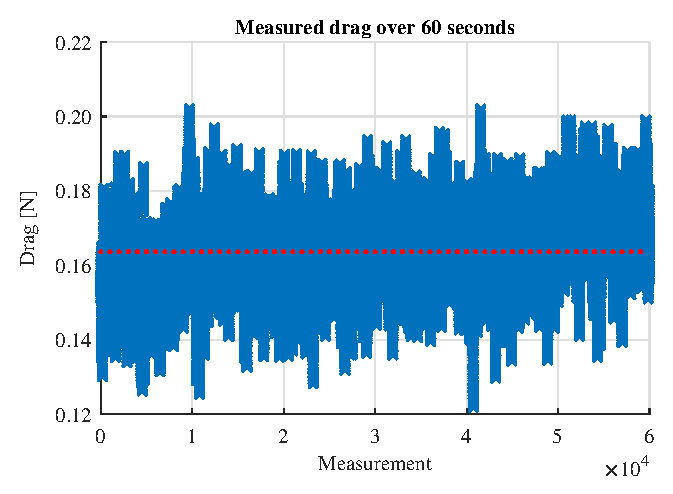
\includegraphics[width=\linewidth]{0_Images/NoiseFirst.eps}
    \caption{The drag for the solid disk at 5 m/s.}
    \label{fig:Noise}
\end{figure}

Figure \ref{fig:Noise} shows each measured drag value at a sampling rate of 1000 Hz over the course of 60 seconds. The measured drag varies with a 0.012, compared to an average of 0.1636. This means that the noise is of one order less that the average. 

This noise may both be related to measurement noise in the force plate, and electrical noise as the signal passes from the force plate, through the amplifier and the lowpass filter. It is still a reasonable assumption that the measurements have a Gaussian distribution and that the average drag is representative. 

The measured temperature only varies between about 20\degree C and 23\degree C. Since this variation is fairly small, it is assumed to not have any significant impact on the resulting drag. 



%Error, standard deviation 

%why do we get the results that we get? 

%- Adjusting for drift 
%- statistikk arument 
%- usikkerhet



